\documentclass[12pt]{article}
\usepackage[left=1cm, right=1cm, top=2cm,bottom=1.5cm]{geometry} 

\usepackage[parfill]{parskip}
\usepackage[utf8]{inputenc}
\usepackage[T2A]{fontenc}
\usepackage[russian]{babel}
\usepackage{enumitem}
\usepackage[normalem]{ulem}
\usepackage{amsfonts, amsmath, amsthm, amssymb, mathtools}

\usepackage{fancyhdr}
\pagestyle{fancy}
\renewcommand{\headrulewidth}{1.5pt}
\renewcommand{\footrulewidth}{1pt}

\usepackage{graphicx}
\usepackage[figurename=Рис.]{caption}
\usepackage{subcaption}
\usepackage{float}

%%Наименование папки откуда забирать изображения
\graphicspath{ {./images/} }

%%Изменение формата для ввода доказательства
\renewcommand{\proofname}{$\square$  \nopunct}
\renewcommand\qedsymbol{$\blacksquare$}

\addto\captionsrussian{%
	\renewcommand{\proofname}{$\square$ \nopunct}%
}
%% Римские цифры
\newcommand{\RN}[1]{%
	\textup{\uppercase\expandafter{\romannumeral#1}}%
}

\theoremstyle{definition}
\newtheorem{defn}{Опр:}
\newtheorem{rem}{Rm:}
\newtheorem{prop}{Утв.}
\newtheorem{exrc}{Упр.}
\newtheorem{lemma}{Лемма}
\newtheorem{theorem}{Теорема}
\newtheorem{corollary}{Следствие}
\newenvironment{cusdefn}[1]
{\renewcommand\thedefn{#1}\defn}
{\enddefn}

\DeclareRobustCommand{\divby}{%
	\mathrel{\text{\vbox{\baselineskip.65ex\lineskiplimit0pt\hbox{.}\hbox{.}\hbox{.}}}}%
}

\newcommand{\smallerrel}[1]{\mathrel{\mathpalette\smallerrelaux{#1}}}
\newcommand{\smallerrelaux}[2]{\raisebox{.1ex}{\scalebox{.75}{$#1#2$}}}
\newcommand{\smallin}{\smallerrel{\in}}
\newcommand{\smallnotin}{\smallerrel{\notin}}


\begin{document}
\lhead{Математический анализ - I}
\chead{Шапошников С.В.}
\rhead{Лекция - 5}
	
\section*{Свойства счетных множеств}
\begin{enumerate}[label={(\arabic*)}]
	\item $B \subset A$ и $A$ - счетно, то $B$ не более, чем счетно (н.б.ч.с);
	\item Если $A$ - счетно и $B$ - счетно, то $A\times B$ - счетно;
	\item Объединение не более, чем счетного набора не более, чем счетных множеств - не более, чем счетно;
	\item Если $A$ - бесконечно, то $\exists$ счетное $B \colon B \subset A$;
\end{enumerate}

\begin{prop}
Если $A$ - счетно, то:\\
	1) если существует инъекция $f \colon B \rightarrow A$, то $B$ - н.б.ч.с.;\\
	2) если существует сюръекция $f \colon A \rightarrow B$, то $B$ - н.б.ч.с.;
\end{prop}

\begin{proof}
	1) $f \colon B \rightarrow \underbrace{f(B)}_\text{обл. знач f}$ - биекция и $f(B) \subset A$ - счетно $\Rightarrow f(B)$ - н.б.ч.с. $\Rightarrow B$ - н.б.ч.с. по определению.\\
	2) Опредлим отображение $g \colon B \rightarrow A$ следующим образом:\\ 
	$$\forall b \in B,\, \exists k \in K = \{\,a \colon f(a) = b \,\} \neq \varnothing \colon g(b) = k,$$ где множество $K$ непустое, так как у нас сюръекция. Так как $f$ - функция, то $g$ - инъекция. Применяя пункт 1) получим, что $B$ - н.б.ч.с.
\end{proof}
\begin{figure}[H]
	\centering
	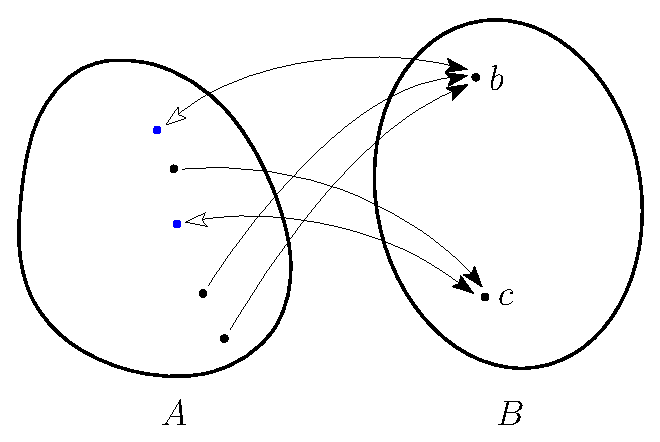
\includegraphics[width=0.45\textwidth]{5_1.eps}
	\caption{Сюръекция}
	\label{5_1}
\end{figure}

\begin{rem}
\uline{Комментарий к доказательству}:\\
$B \neq \varnothing$ и на $B$ есть cюръекция $\Leftrightarrow$ у каждого элемента $B$ есть прообраз, но он может быть не один (не инъективно). $\forall b \in B$ укажем тот $a$ (выделено синим на рисунке), куда будем возвращаться.\\ 
Разным элементам из $B$, точно не будут соответствовать одни и те же элементы из прообраза, иначе $f$ могло бы отображать один элемент в несколько, а $f$ - это функция и каждому сопостовляет ровно 1 элемент $\Rightarrow$ разным $b$ и $c$ будут соответствовать разные элементы из $A$. 
Поэтому из $B$ в $A$ установили инъекцию $\Rightarrow$ по первому пункту $B$ - н.б.ч.с.
\end{rem}

\newpage
\subsection*{Счетность декартовых произведений}

(2) Если $A$ - счетно и $B$ - счетно, то $A\times B$ - счетно.
\begin{proof}
Можно пересчитывать по диагонали: справа - налево, сверху - вниз.\\
Пусть стоит клетка на пересечении $k$-ой строки и $l$-го столбца. Она стоит на диагонали с номером $k+l-1$.
Последняя клетка на $n$-ой диагонали имеет номер: $1 + 2 + 3 + \dotsc + (n-1) + n = \dfrac{n(n+1)}{2}$. 

$2$-ая диагональ $\Rightarrow$ последний элемент $= 1 + 2 = 3$, $3$-ья диагональ $\Rightarrow$ последний элемент $= 1 + 2 + 3 = 6$.

	\begin{figure}[H]
		\centering
		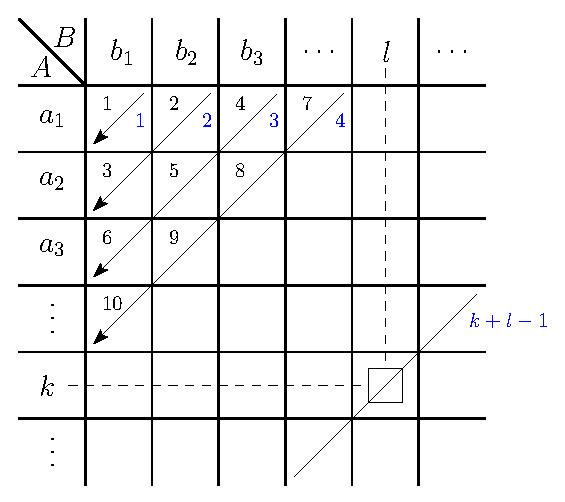
\includegraphics[width=0.5\textwidth]{5_2.eps}
		\caption{Метод пересчета по диагонали}
		\label{5_2}
	\end{figure}

Если считать по столбцам, то $(k, l)$ элемент отстоит от $1$-го столбца на $(l-1)$ шаг $\Rightarrow$ присвоим номер клетке
$$(k,l) \mapsto \dfrac{(k+l-1)(k+l)}{2} - (l-1),$$
как число шагов вправо от последнего номера на диагонали $\Rightarrow$ получили явную формулу, устанавливающую биекцию $A\times B \mapsto \mathbb{N}$.
\end{proof}

\begin{corollary}
$A_1, \dotsc, A_n$ - счетные множества, то $A_1 \times \dotsc \times A_n$ - счетное множество (доказательство по индукции).
\end{corollary}

\subsection*{Счетность объединения множеств}

(3) Объединение н.б.ч.с. набора н.б.ч.с. множеств - н.б.ч.с.
\begin{proof}
Пусть есть множество $A_\alpha = \{\, a_{\alpha\beta} \mid \beta \in \text{J}_\alpha \text{ - н.б.ч.с.}\,\}$, где $\alpha \in \text{I}$ - н.б.ч.с. множество. Покажем, что $\bigcup\limits_{\alpha \smallin \text{I}} A_\alpha$ - не более, чем счетно. Если множество н.б.ч.с., то существует сюръекция из $\mathbb{N}$ в это множество:\\
(a) Если множество счетное, то существует биекция. 
 \begin{figure}[H]
	\centering
	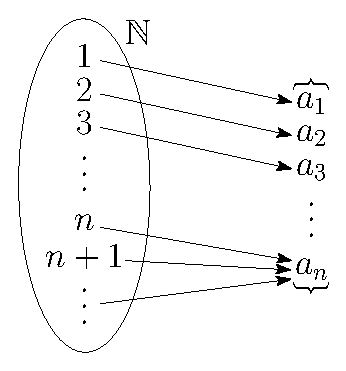
\includegraphics[width=0.2\textwidth]{5_3.eps}
	\caption{Сопоставление $\mathbb{N}$ конечному множеству}
	\label{5_3}
\end{figure}
(b) Если множество конечное, то отображение на первые $n$ элементов - биекция, оставшиеся куда-то переводятся $\Rightarrow$ получается сюръекция. 

Тогда есть сюръекция $f \colon \underset{\text{сюръекция}}{\mathbb{N} \rightarrow \text{I}}$. Также $\forall \alpha,\, A_\alpha = \{\,a_{\alpha\beta} \mid \beta \in \text{J}_\alpha \text{ - н.б.ч.с.}\,\}$ поэтому для каждой $\alpha$ сюръекция будет своя $g_\alpha \colon \underset{\text{сюръекция}}{\mathbb{N} \rightarrow \text{J}_\alpha}$.\\ 
Установим отображение $$\mathbb{N}\times \mathbb{N} \mapsto \bigcup\limits_{\alpha  \smallin \text{I}} A_\alpha,$$ как $(n,m) \mapsto  a_{f(n)g_{f(n)}(n)}$ - сюръекция $\Rightarrow$ объединение - н.б.ч.с. по утверждению выше.
\end{proof}
\uline{Объяснение для детей}: пересчитываем по диагонали, если элемент был посчитан - не считаем, если считать нечего - то тоже не считаем.
\begin{figure}[H]
	\centering
	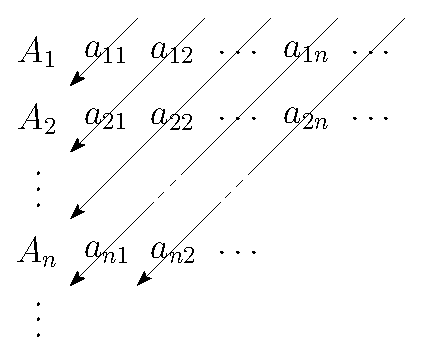
\includegraphics[width=0.25\textwidth]{5_4.eps}	
	\caption{Пересчет объединения н.б.ч.с набора н.б.ч.с. множеств}
	\label{5_4}
\end{figure}
Либо все элементы закончатся, либо будуте считать бесконечно долго и получим бесконечно долгий пересчет. Формальное доказательство - то же самое что и здесь.

\textbf{Пример:} Множество рациональных чисел $\mathbb{Q} \subset \mathbb{Z} \times \mathbb{N}$ - счетно, так как: $\mathbb{Z}$ - счетное множество, $\mathbb{N}$ - счетное множество $\Rightarrow$ декартово произведение - счетно $\Rightarrow \mathbb{Q}$ - н.б.ч.с. Так как $\mathbb{N} \subset \mathbb{Q} \Rightarrow \mathbb{Q}$ - счетно.

(4) Если $A$ - бесконечно, то $\exists$ счетное $B \colon B \subset A$.
\begin{proof}
	Поскольку $A$ - не является конечным, то $A \neq \varnothing$, $a_1 \in A$. $A \setminus \{a_1\} \neq \varnothing$ - поскольку $A$ не является конечным $\Rightarrow a_2 \in A\setminus\{a_1\}, \dotsc,\, a_{n+1} \in A \setminus\{a_1, ... , a_n\} \Rightarrow$ получили набор $\{a_n\} \subset A$: для разных номеров - это различные элементы $\Rightarrow$ установлена биекция между этим набором и $\mathbb{N}$.
\end{proof}

\begin{exrc}
	 Если $A$ - бесконечное и $C$ - счетное, то $A \cup C \sim A$.
\end{exrc}
 
\subsection*{Пример Кантора}
$\{0,1\}^{\infty}$ - множество всех бесконечных последовательностей из 0 и 1. 

\begin{prop}
	Множество $\{0,1\}^{\infty}$ - не является счетным.
\end{prop}
\begin{proof}
(От противного): Предположим, что можно занумеровать эти последовательности натруальными числами: $\RN{1}\colon 0110\dotsc;\, \RN{2}\colon 1110\dotsc;, \, \dotsc,\, n\colon \dotsc;$.
Возьмем такую последовательность: $1$-ый элемент из $1$-ой последовательности, $2$-ой элемент из $2$-ой последовательности, $\dotsc$, $n$-ый элемент из $n$-ой последовательности и так далее.

Возьмем отрицание данной последовательности, то есть: $0 \rightarrow 1$ и $1 \rightarrow 0$.\\
Этой последовательности в списке нет, поскольку на $1$-ом месте у нее находится не то, что у $1$-ой последовательности, на $2$-ом месте - не то, что у $2$-ой, на $n$-ом месте - не то, что у $n$-ой и так далее $\Rightarrow$ от каждой в списке отличается в диагональном элементе $\Rightarrow$ такой последовательности нет $\Rightarrow$ для любого пересчета будет указана последовательность, которая там не находится.
\end{proof} 

\section*{Теорема Кантора-Берштейна}

\begin{theorem}
	\textbf{(Кантора Берштейна)}: Если $A \sim B' \subset B$ и $B \sim A' \subset A \Rightarrow A \sim B$.
\end{theorem} 

\begin{proof}
	
\begin{figure}[H]
	\centering
	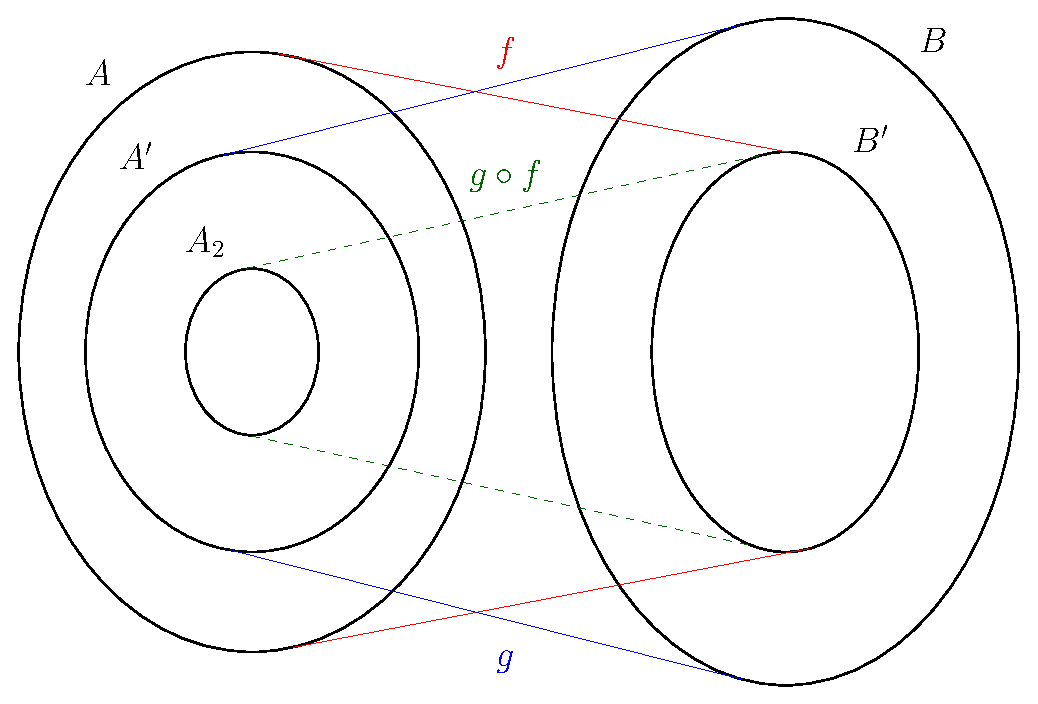
\includegraphics[width=0.55\textwidth]{5_5.eps}
	\caption{Отображения множеств: $f \colon A \rightarrow B', \, g \colon B \rightarrow A', \, g \circ f \colon A \rightarrow A_2$}
	\label{5_5}
\end{figure}	

Множество $A$ биективно отображается на $B'$, множество $B$ биективно отображается на $A'$. Возьмем композицию этих отображений. Композиция биекций - это биекция, поэтому мы можем заключить, что $A \sim A_2$. 
$$f \colon A \rightarrow B', \, g \colon B \rightarrow A', \, g \circ f \colon A \rightarrow A_2$$
Перерисуем картинку следующим образом: множества $A_0 =A$, $A_1 = A'$ и $A_2 = A_2$. 

\begin{figure}[H]
	\centering
	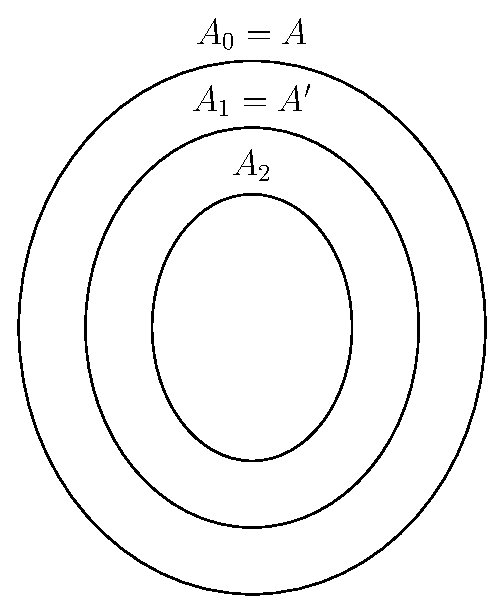
\includegraphics[width=0.25\textwidth]{5_6.eps}	
	\caption{Разбиение исходного множества $A$} 
	\label{5_6}
\end{figure}		
Идея: $A_2 \subset A_0$ и $A_2 \sim A_0$ значит все, что находится между ними также должно быть равномощно $A_0 = A$. Зная, что $A_0 \sim A_2$ хотим показать, что $A_0 \sim A_2 \Rightarrow A_0 \sim A_1$, тогда $A \sim A' \sim B \Rightarrow A \sim B$.

\begin{figure}[H]
	\centering
	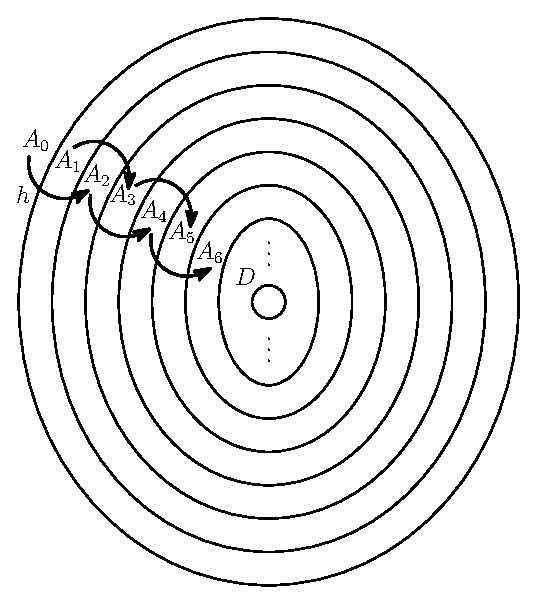
\includegraphics[width=0.35\textwidth]{5_7.eps}	
	\caption{Построение множеств $A_{2n+1}$ и $A_{2n}$} 
	\label{5_7}
\end{figure}	

Есть биекция $h \colon A_0 \rightarrow A_2$. Она же переводит $A_1$ в некое множество, пусть: $A_3 = h(A_1)$.\\
В множестве $A_1$ есть $A_2 \Rightarrow A_2 \subset A_0 \Rightarrow$ биекция переводит $A_2$ в некое множество $A_4 = h(A_2)$.\\
Продолжаем по аналогии и получаем: $A_5 = h(A_3), \, A_6 = h(A_4), \dotsc \, $, и так далее. Обозначим центр, как $D$ он может быть пустым. Получим:

$$A_{2n+1} = h(A_{2n-1}), \, A_{2n} = h(A_{2n-2})$$

Построим следующие множества: $C_0 = A_0 \setminus A_1$, $C_1 = A_2 \setminus A_3$.\\ 
Проверим, что $C_0 \sim C_1$: $A_0 \xrightarrow{h} A_2$ - биекция, $A_0 \supset A_1 \xrightarrow{h} A_3 \subset A_2$ - биекция $\Rightarrow$ поскольку $h$ - биекция, то $h\colon A_0 \setminus A_1 \rightarrow A_2 \setminus A_3 \Rightarrow C_0 \sim C_1$.

\begin{figure}[H]
	\centering
	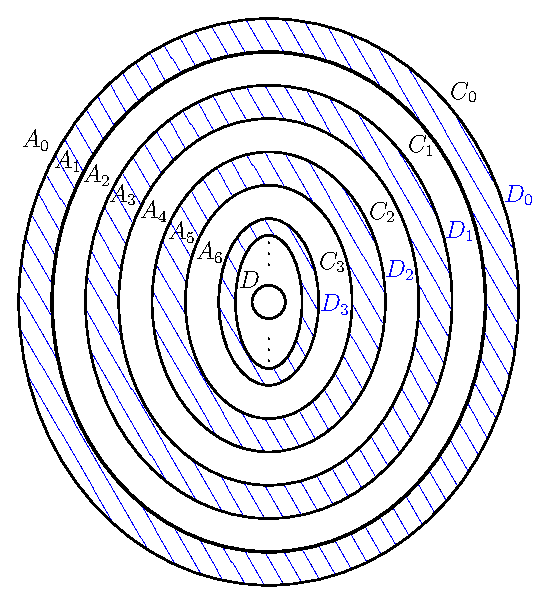
\includegraphics[width=0.35\textwidth]{5_8.eps}	
	\caption{Построение множеств $C_{m}$ и $D_{k}$} 
	\label{5_8}
\end{figure}

Далее построим следующие множества: $C_1 = A_2 \setminus A_3, \, C_2 = A_4 \setminus A_5$.\\
Покажем, что $C_1 \sim C_2$, аналогично проверенному: $A_2 \xrightarrow{h} A_4$ - биекция, $A_2 \supset A_3 \xrightarrow{h} A_5 \subset A_4$ - биекция $\Rightarrow$ поскольку $h$ - биекция, то $h\colon A_2 \setminus A_3 \rightarrow A_4 \setminus A_5 \Rightarrow C_1 \sim C_2$.

И так далее по аналогии. Получим биекцию $h$ которая переводит эти слои друг в друга: 
$$C_1 \xrightarrow{h} C_2 \xrightarrow{h} C_3 \xrightarrow{h} \dotsc$$

Поскольку слоев бесконечно много, то первый слой биективно перекладываем внутрь. Таким образом - все закрашенные круги сдвигаются внутрь, а все незакрашенные (обозначим их, как $D_k$) остаются на месте:
$$A_0 = C_0 \cup D_0 \cup C_1 \cup D_1 \cup \dotsc \cup D$$
$$A_1 = D_0 \cup C_1 \cup D_1 \cup \dotsc \cup D$$
Устанавливаем биекцию $F \colon D_i \rightarrow D_i$, $F \colon C_i \rightarrow C_{i+1}$. Множества попарно не пересекаются и для каждого установлен переход $\Rightarrow A_0 \rightarrow A_1$ - биекция.
\end{proof}

\section*{Теорема Кантора}

\begin{theorem}
	$A \nsim 2^A$
\end{theorem}
\begin{proof}
	Предположим противное, что $\exists f \colon A \rightarrow 2^A$ - биекция. Тогда по этому отображению $a \rightarrow f(a)$, где $f(a)$ - множество.
	Рассмотрим множество $C = \{\,a \colon a \notin f(a)\,\} \subset A$ - это те элементы $a$, образ которых их не содержит. Так как $C \subset A$, то по построению $\exists b \in A \colon f(b) = C$, поскольку у нас биекция.\\
	В случае $b \in f(b) = C \Rightarrow b \notin f(b)$ - противоречие. В случае $b \notin f(b) \Rightarrow b \in C = f(b)$ - противоречие.\\ 
	Поэтому не существует такой биекции $\Rightarrow$ множества не равномощны. 
\end{proof}
 \begin{exrc}
 	Сравнить с парадоксом Рассела.
 \end{exrc}
 
 В $2^A$ есть набор подмножеств, вида $\{a\}$  - одноэлементные подмножества, где $a \in A$. Этот набор отождествляется с $A$ или равномощен $A$. Таким образом 
 $A \sim C \subset 2^A$, но $A \nsim 2^A \Leftrightarrow A$ - меньше по мощности, чем множество всех подмножеств $2^A$. 
 
\begin{rem}
	Множество всех подмножеств $\mathbb{N}$ не может быть счетным по теореме Кантора: $2^{\mathbb{N}} \nsim \mathbb{N}$.
\end{rem} 

Данный пример ничем не отличается от предыдущего примера про несчетные множества:\\ 
Возьмем последовательность $B \in 2^{\mathbb{N}}$, состоящую из $0$ и $1$. Выпишем последовательность натуральных чисел $1, 2, \dotsc, n, \dotsc$ и будем ставить $1$ если $n \in B$ и $0$ если $n \notin B$. Таким образом напротив каждого натурального числа будет $0$ или $1$. Следовательно есть биекция: $2^{\mathbb{N}} \sim \{0,1\}^{\infty}$.
 \begin{exrc}
 	Сравнить обоснование примера Кантора и доказательства теоремы Кантора.
 \end{exrc}
 
\end{document}